%Nous avons utilisé Git dès le début du projet, sachant qu'en plus c'est l'un des gestionnaires de version le plus performant son utilisation était évidente.
Afin de permettre une meilleure gestion de projet (travail parallèle, gestion de bug, etc.) nous avons décidé d'utiliser le gestionnaire de version Git ainsi que le service GitLab mis à la disposition des étudiants par le SIF.
La prise en main fut facile, les membres du groupe ayant tous déjà utilisé cet outil. Nous avons ainsi utilisé le système de suivi de bug intégré à Gitlab (cf. Figure~\ref{bugs}).

\begin{figure}[h]
\centering
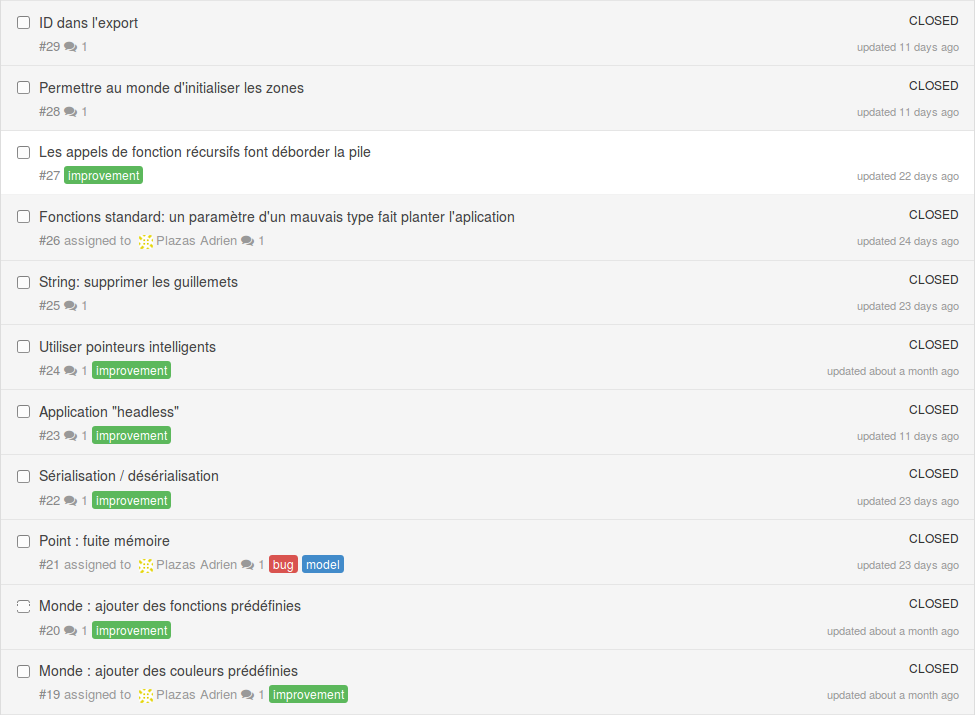
\includegraphics[scale=0.35]{doc/gestionProjet/bugs.png}
\caption{\label{bugs} Système de suivi de bugs de Gitlab}
\end{figure}

%Git permet de travailler séparement sans soucis. La prise en main s'est faite assez facilement car nous connaissions déjà cet outil, cela nous a donc permis d'en faire une utilisation plus poussée pour en avoir une meilleure gestion (utilisation de branches, des issues, etc).
%Nous avons installé un dépôt sur le GitLab du Sif, service 

%Nous avons utilisé une branche Master, qui devait contenir uniquement du code compilable, et après, chaque fonctionnalité a été développé sur une branche différente.
Notre organisation des branches fut la suivante~:
\begin{itemize}
\item la branche master devait contenir une version fontionnelle compilable~;
\item des branches de développement étaient créées pour chaque nouvelle fonctionnalité, et n'étaient fusionnées que lorsqu'elles étaient pleinement fonctionnelles~;
\item des branches «~tags~» ont été créées pour les différentes versions.
\end{itemize}
Nous utilisions également Gitg, pour avoir une meilleure vue de l'état de notre dêpot (cf. Figure~\ref{Gitg}).
\begin{figure}[h]
\centering
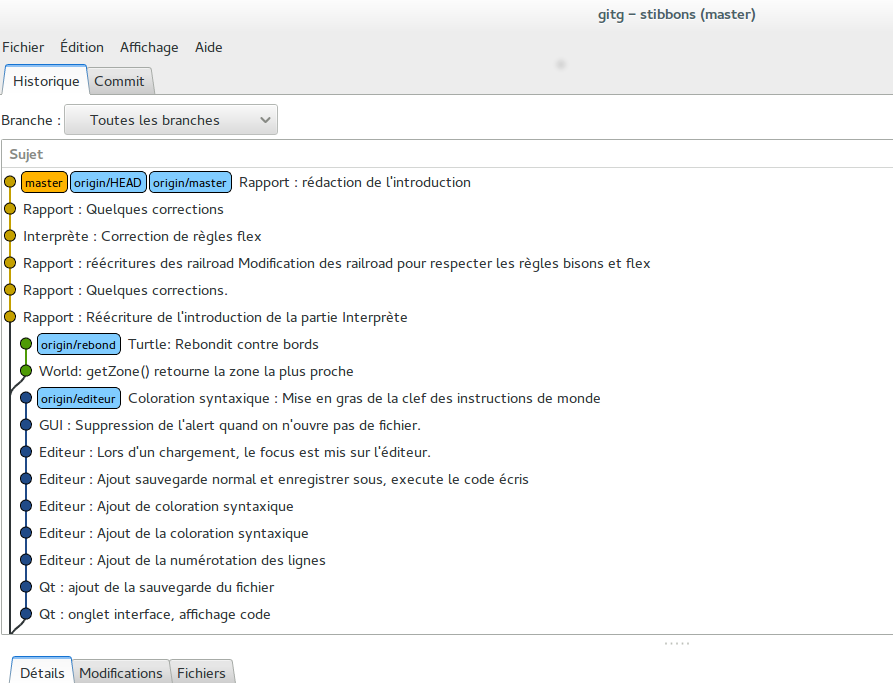
\includegraphics[scale=0.35]{doc/gestionProjet/gitbranche.png}
\caption{\label{Gitg} Gitg}
\end{figure}
% nb de ligne : wc -l `find . -name "*.h"` `find . -name "*.cpp"` `find . -name "*.y\+"` `find . -name "*.l\+"`
Lors de la version 1.0, nous avions 493 commits, avec une moyenne de 4,7 commits par jour, soit 98,6 commits par version en moyenne, 12 branches, 0 tags (nous avons utilisé les branches en guises de label de versions).
Nous avions également au total 11827 lignes de code, réparties en 324 lignes pour l'application console, 1496 lignes pour l'application graphique, 3027 lignes dans la partie interprète, 6188 lignes dans le modèle et 792 lignes de tests.
\begin{figure}[h]
\centering
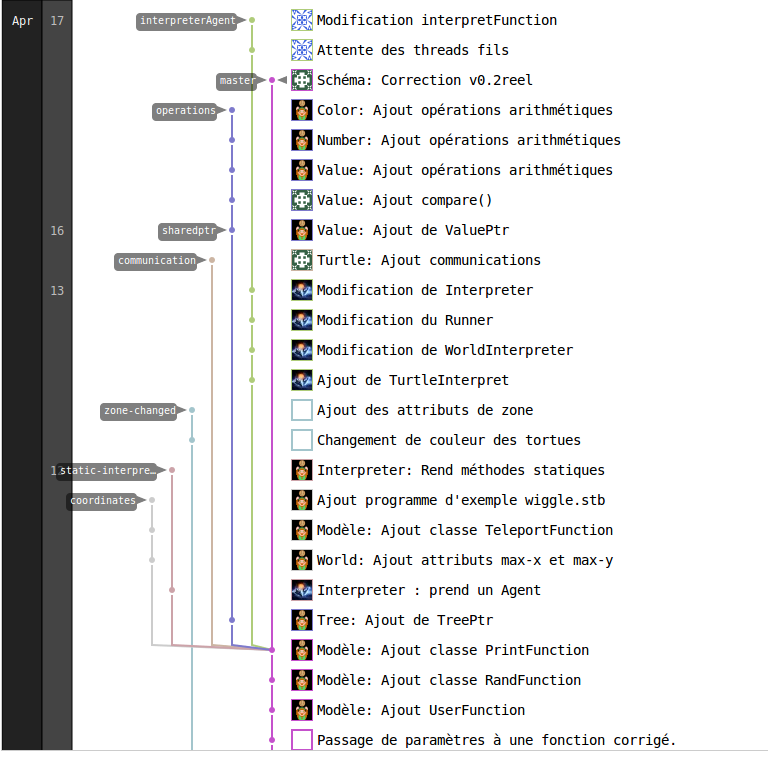
\includegraphics[scale=0.35]{doc/report/uml/network-v3.png}
\caption{\label{branche} Branches lors de la 0.3 sur Gitlab}
\end{figure}

